% !TEX encoding = UTF-8
\setchapterstyle{kao}
\setchapterpreamble[u]{\margintoc}
\chapter{MESURES ET INCERTITUDES}
\labch{mesures_et_incertitudes}


\blockquote[Edgar Morin]{La connaissance progresse en intégrant en elle l'incertitude, non en l'exorcisant}

Accéder à une valeur objective de la réalité sans erreur est tout simplement impossible. L'erreur fait parti de l'opération de mesure. Une des forces de la science est d'avoir mis au point des outils qui permettent d'\textbf{estimer} cette erreur.

\begin{center}
\textbf{Version en ligne}

\url{https://femto-physique.fr/omp/mesures-et-incertitudes.php}
\end{center}





\section{Mesurer c'est évaluer}%(fold)

\subsection{Notion d'erreur et d'incertitude}[Erreur et incertitude]%(fold)
\begin{kaoexample}[frametitle=Expérience]
Mesurons, à l'aide d'un chronomètre, la durée $t$ correspondant à 2,5 périodes d'oscillation d'un pendule simple (5 passages à la verticale). En faisant faire cette même mesure par différents élèves on trouve 
\begin{center}
\begin{tabular}{c|cccc}
mesure \no&1&2&3&4\\
\hline
durée $t$&3,62~s&3,47~s&3,44~s&3,30~s\\
\end{tabular}	
\end{center}
\end{kaoexample} 
L'expérience précédente montre que les résultats sont différents ce qui traduit l'existence \textbf{d'erreurs de mesure}.  L'erreur faite lors de la mesure d'une grandeur $x$ est l'écart entre la valeur mesurée ($x_i$) et sa valeur vraie ($x_\text{vraie}$), laquelle est unique mais inaccessible. Elle présente deux composantes.
\begin{description}
	\item[Erreur aléatoire] L'erreur aléatoire $\epsilon_a$ provient des variations temporelles et spatiales \textbf{non prévisibles} de grandeurs d'influence\sidenote{Par exemple, le soin avec lequel sont effectuées les mesures, la température de la pièce, la fidélité de l'appareil de mesure, etc.}. Elle est définie par  
	\[\epsilon_a=x_i-\overline{x}\]
	où $\overline{x}$ est la moyenne des mesures obtenue en répétant $N$ fois la même expérience avec $N\to \infty$.
	\item[Erreur systématique] L'erreur systématique\sidenote{On dit aussi \emph{biais}.} $\epsilon_s$ est un \textbf{décalage constant} dont l'origine peut être d'ordre théorique ou expérimentale\sidenote{Exemple de biais: influence du mode opératoire, problème de calibrage d'un appareil, modélisation incomplète, etc.}. Par définition, 
	\[
	\epsilon_s=\overline{x}-x_\text{vraie}
	\]
Ainsi, l'erreur sur une mesure est la somme d'un biais et d'une quantité aléatoire :
	\[
	\epsilon=x_i-x_\text{vraie}=(x_i-\overline{x})+(\overline{x}-x_\text{vraie})=\epsilon_a+\epsilon_s
	\]
\end{description}

\begin{kaoexample}[frametitle=Exemple]
Dans l'expérience précédente on peut lister les différentes sources d'erreur :
\begin{center}
	\begin{tabular}{l|l}
	% \toprule
	\textbf{Erreur aléatoire}		& \textbf{Erreur systématique (biais)}\\
	\midrule
	réflexe humain					& défaut de parallaxe\\
	fidélité limité du chronomètre	&	chronomètre mal calibrés\\
	erreur de lecture				&	verticale mal positionnée\\				 
	% \bottomrule
	\end{tabular}
\end{center}
\end{kaoexample} 
\begin{kaobox}[frametitle=Correction d'un biais]
Bien qu'il ne soit pas possible de compenser l'erreur aléatoire faite sur une mesure, elle peut être réduite en augmentant le nombre d'observations comme nous allons le voir. En revanche, l'erreur systématique d'un résultat de mesure ne peut être réduite en augmentant le nombre d'observations, mais par l'application d'une \textbf{correction}.
\end{kaobox}

Le résultat final est exprimé sous la forme d'un \textbf{intervalle de valeurs probables}
\[
x=x_\text{m} \pm \Delta x
\]
où $x_\text{m}$ est la mesure, c'est-à-dire la meilleure estimation de la valeur vraie et $\Delta x$ l'\textbf{incertitude sur la mesure} que l'on cherche à évaluer. Plus précisément l'intervalle $[x_\text{m}-\Delta x,x_\text{m}+\Delta x]$ est défini comme un intervalle de confiance associé à une probabilité de contenir la valeur vraie $x_\text{vraie}$. Cette probabilité est appelé \textbf{niveau de confiance}.

\begin{kaoexample}[frametitle=Exemple]
La masse de l'électron vaut (CODATA 2010)
\[
m_\text{e}=(9,109 382 91\pm 0,000 000 40)\cdot 10^{-31}\;\mathrm{kg}	
\]
avec un niveau de confiance de 68\%.
\end{kaoexample} 

Insistons sur le fait que sans incertitude il nous est impossible de comparer deux résultats ou de réfuter une loi. Pour qu'un résultat ait une valeur scientifique il faut pouvoir prouver que les éventuels écarts entre la théorie et l'expérience sont non significatifs c'est-à-dire liés aux erreurs de mesure ce qui rend nécessaire l'estimation des incertitudes. 
%(end)
\subsection{Écriture scientifique}%(fold)
Avant de voir comment estimer les incertitudes, faisons une petite mise au point sur les conventions d'écriture scientifique. 

Dans une valeur numérique, le premier chiffre non-nul de gauche désigne le chiffre le plus significatif et le dernier chiffre de droite le chiffre le moins significatif. Les nombres 1230, 1,230 et 0,001230 ont ainsi tous quatre chiffres significatifs. Le nombre de chiffres significatifs rend compte de la précision du résultat et permet donc de se faire une idée de l'incertitude, même quand cette dernière n'est pas indiquée. Par exemple, écrire	
\[
c = (3,00278\pm 0,04)\cdot 10^{8}\,\mathrm{m.s^{-1}}
\]
n'a aucun sens, puisque l'incertitude indique que nous n'avons pas d'information au delà de la deuxième décimale. Il faut donc arrondir le résultat au centième.
\begin{kaobox}[frametitle=Comment arrondir ?]
Pour les arrondis on adopte la méthode qui consiste à arrondir au plus près : cela consiste à repérer le dernier chiffre à arrondir (en fonction de la précision) puis à l'augmenter d'une unité si le chiffre suivant est au moins égal à 5 ou à le conserver sinon. Par exemple, 
\begin{itemize}
	\item arrondir 1,645 à l'unité donne 2 ;
	\item arrondir 1,645 au dixième donne 1,6 ;
	\item arrondir 1,645 au centième donne 1,65.
\end{itemize}
\end{kaobox}
Si l'on reprend l'exemple précédent, on écrira plutôt 
\[
c = (3,00\pm 0,04)\cdot 10^{8}\,\mathrm{m.s^{-1}}
\]
Par ailleurs, l'incertitude étant elle-même entachée d'une incertitude assez importante, on ne garde qu'un seul chiffre significatif, éventuellement deux si l'on estime faire une erreur d'arrondi trop importante avec un seul chiffre. Par exemple
\[	
175,652\pm 6,922\to176\pm7	\quad\text{et}\quad	175,652\pm 1,394\to175,7\pm1,4	
\]
\begin{kaobox}[frametitle=En résumé]
Une fois l'incertitude estimée, on l'arrondit à un ou deux chiffres. On ajuste la valeur de la mesure $x_\text{m}$ de manière à ce que son \textbf{dernier chiffre significatif soit à la même position que celui de l'incertitude} en arrondissant au plus près. Le résultat se met sous la forme 
\[
x=(x_\text{m}\pm\Delta x)\cdot 10^n\quad\text{unité}
\]
\end{kaobox}
%(end)

%(end)

\section[Estimation d'une incertitude]{Comment estimer une incertitude ?}%(fold)
Décrivons les différentes méthodes qui nous permettent d'évaluer les erreurs aléatoires. Notez que l'on suppose les erreurs systématiques négligeables et que ça n'est qu'à la fin, lorsque l'on confronte théorie et expérience, que l'on peut invoquer l'existence de biais pour expliquer un désaccord. 

\subsection{Généralités}%(fold)
\begin{marginfigure}
\centering
\centering
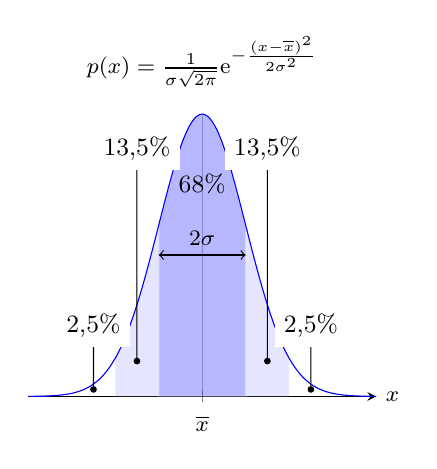
\begin{tikzpicture}
\def \xMoy{5};%moyenne
\def \ecartType {1};%ecart-type
	\begin{axis}[
	width=6cm,
	grid=major,
	hide y axis,
	axis lines=middle,%none,bottom,top
	inner axis line style={=>},
	title={$p(x)=\frac{1}{\sigma \sqrt{2\pi}}\mathrm{e}^{-\frac{(x-\overline{x})^{2}}{2\sigma^{2}}}$},
	xlabel={$x$},
	xlabel style={anchor=west},
	xtick={5},
	xticklabels={$\overline{x}$},
	x tick label style={below=0.5mm},
	ytick=\empty,
	xmin=1,
	xmax=9,
	ymin=0,
	ymax=0.4,
	font=\footnotesize,
	]
	\addplot+[thick,mark=none,fill=blue,draw=white,opacity=0.1,domain=3:7,samples=150] {(exp(-(x-\xMoy)^2/(2*\ecartType^2)))/(\ecartType*sqrt(6.28))}\closedcycle;
	
	\addplot+[thick,mark=none,fill=blue,draw=white,opacity=0.2,domain=4:6,samples=150] {(exp(-(x-\xMoy)^2/(2*\ecartType^2)))/(\ecartType*sqrt(6.28))}\closedcycle;
	\addplot+[draw=blue,mark=none,domain=1:9,samples=200]{(exp(-(x-\xMoy)^2/(2*\ecartType^2)))/(\ecartType*sqrt(6.28))};
	
	\draw[<->] (axis cs:4,0.2)--(axis cs: 6,0.2) node[midway,above]{$2\sigma$};
	\draw (axis cs:5,0.3) node{\small 68\%};
	\draw[fill=black] (axis cs:6.5,0.35) node[fill=white]{\small 13,5\%}--(axis cs:6.5,0.05)circle[radius=1pt];
	\draw[fill=black] (axis cs:3.5,0.35) node[fill=white]{\small 13,5\%}--(axis cs:3.5,0.05)circle[radius=1pt];
	\draw[fill=black] (axis cs:7.5,0.1) node[fill=white]{\small 2,5\%}--(axis cs:7.5,0.01)circle[radius=1pt];
	\draw[fill=black] (axis cs:2.5,0.1) node[fill=white]{\small 2,5\%}--(axis cs:2.5,0.01)circle[radius=1pt];
	\end{axis}
\end{tikzpicture}
\caption[Distribution gaussienne]{Loi de probabilité d'une variable aléatoire gaussienne. On a 68\% de chance de trouver $x$ dans l'intervalle $\overline{x}\pm\sigma$ et 95\% dans l'intervalle $\overline{x}\pm2\sigma$.}
\labfig{gaussienne}
\end{marginfigure}
Finalement, mesurer c'est accéder à une grandeur aléatoire. Cette variable aléatoire présente une distribution qui a souvent l'allure d'une gaussienne dont la figure \reffig{gaussienne} en donne une représentation.

Pour caractériser la dispersion des résultats autour de la moyenne on définit \textbf{l'écart-type} $\sigma$ : 
\[
	\sigma\stackrel{\text{def}}=\sqrt{\overline{(x-\overline{x})^2}}
\]
où $\overline{x}$ désigne la moyenne\sidenote{On dit \emph{espérance} en mathématique.} et $\overline{(x-\overline{x})^2}$ la moyenne des écarts quadratiques. On montre qu'il existe une probabilité de 68\% pour qu'une mesure soit compris dans l'intervalle $\overline{x}\pm\sigma$. On dit alors que l'intervalle $\overline{x}\pm\sigma$ représente un niveau de confiance de 68\%. Le problème que l'on se pose est, comment, à partir de mesures, évaluer les valeurs $\overline{x}$ et $\sigma$ ?

Pour cela, il existe deux types d'estimations : 
\begin{description}
	\item[Type A --] On répète $n$ fois la même expérience puis on effectue une analyse statistique.
	
	\item[Type B --] À partir d'une seule mesure on estime $\overline{x}$ et $\sigma$ à l'aide de différentes informations (notices techniques) et d'hypothèses probabilistes.
\end{description}
%(end)
\subsection{Estimation de type A}%(fold)
Supposons que l'on collecte $n$ mesures en répétant $n$ fois la même expérience. On cherche à accéder aux paramètres $\overline{x}$ et $\sigma$ à partir des $n$ mesures $x_1$, $x_2$, ..., $x_n$. Si $n\to \infty$ on pourrait reconstruire la loi de probabilité relative  à la variable $x$ et par conséquent calculer $\overline{x}$. Hélas, $n$ est fini ; il faut donc chercher la meilleur façon d'estimer les paramètres $\overline{x}$ et $\sigma$ à partir d'un ensemble discret de mesures.

Nous distinguerons  deux situations : 
\begin{itemize}
	\item le cas où l'échantillon de mesures est grand,  disons $n\geq10$ ;	
	\item le cas où l'échantillon est petit, c'est-à-dire $n<10$.
\end{itemize}

\subsubsection{Cas où $n\geq10$}
La théorie des probabilités permet de montrer que la meilleur estimation de $\overline{x}$ est la \textbf{moyenne arithmétique}.
% --- equation --- (fold)
\begin{equation}
\fcolorbox{filet}{fond}{\hspace{0.5em}
\(\displaystyle 
m\stackrel{\text{def}}= \dfrac{x_1+x_2+\cdots+x_n}{n}\simeq \overline{x}
\)\hspace{0.5em}}
\hspace{0.5em}\heartsuit
\label{eq:moyenne_arithmetique}
\end{equation}
%--- equation --- (end)
On montre également que la meilleure estimation de $\sigma$ est \textbf{l'écart-type non biaisé} (noté $\sigma_{n-1}$ sur les calculatrices)
% --- equation --- (fold)
\begin{equation}
\fcolorbox{filet}{fond}{\hspace{0.5em}
\(\displaystyle 
s\stackrel{\text{def}}=\sqrt{\frac{(x_1-m)^2+(x_2-m)^2+\cdots+(x_n-m)^2}{n-1}}\simeq \sigma
\)\hspace{0.5em}}
\hspace{0.5em}\heartsuit
\label{eq:ecart_type_non_biaise}
\end{equation}
%--- equation --- (end)
Notez que dans cette formule, la somme des écarts quadratiques est divisé par $n-1$ et non par $n$ comme on pourrait s'y attendre. Une façon de retenir ce facteur $n-1$ est de réaliser que pour estimer un écart-type il faut au moins deux mesures ce qui implique $n>1$.

\subsubsection{Cas où $n\leq 10$}
Si l'échantillon est petit (disons $n\leq 10$) il y a une correction à apporter. On montre alors que la meilleure estimation de l'écart-type vaut $t\times s$ où $t$ est le \emph{coefficient de Student} donnée dans la \reftab{Coef_students}.
\begin{margintable}
	\caption{Coefficients de Student pour un intervalle de confiance de $68\%$}
	\labtab{Coef_students}
	\footnotesize
	\begin{tabular}{@{}l|c@{}}
	\toprule
	Nombre de mesures $n$&	Coefficient $t$ \\
	\midrule
	2&	1,84\\
	3&	1,32\\
	4&	1,20\\
	5&	1,14\\
	6&	1,11\\
	7&	1,09\\
	8&	1,08\\
	9&	1,07\\
	10&	 1,06\\
	\bottomrule
	\end{tabular}
\end{margintable}
\begin{kaoexample}[frametitle=Exemple]
Dans l'expérience précédente, on peut estimer l'incertitude-type associé à la mesure de la durée $t$. On trouve 
	\[m=\dfrac{3,62+3,47+3,44+3,30}{4}=3,4575\;\mathrm{s}\]
	et puisque l'échantillon contient $n=4$ mesures, 
	\[\sigma_t=
	1,2\times\sqrt{\dfrac{(0,1625)^2+(0,0125)^2+(-0,0175)^2+(-0,1575)^2}{3}}\simeq0,1575\;\mathrm{s}\]
Ainsi, chaque mesure présente une incertitude-type de l'ordre de 0,16~s.
\end{kaoexample} 

\subsubsection{Incertitude sur la moyenne arithmétique}
La moyenne arithmétique est la meilleure estimation de la valeur vraie, pour autant elle n'en est pas moins entachée d'une certaine erreur. En effet, si l'on répète une autre série  de $n$ mesures on trouve une autre valeur de $m$. Il faut donc chercher à calculer l'écart-type de la moyenne $\sigma_m$. Il est alors assez facile de montrer que 
\[
\sigma_m=\frac{\sigma}{\sqrt{n}}\simeq \frac{t\,s}{\sqrt{n}}
\]
En d'autres termes, par rapport à une mesure isolée, on réduit l'incertitude d'un facteur $\sqrt{n}$ en procédant à $n$ mesures\sidenote{On pourrait croire qu'il suffit de procéder à un très grand nombre de mesures pour accéder à la valeur vraie de façon très précise mais ce serait oublier la présence d'erreurs systématiques qui ne s'effacent pas avec le nombre d'observations. À partir d'un certain nombre $n$ l'erreur systématique l'emporte sur l'erreur aléatoire. Toute la difficulté réside alors dans la détermination puis la correction des différents biais, comme nous le rappelle la très médiatique affaire des neutrinos supraluminiques.}. Finalement, le résultat se met sous la forme 
% --- equation --- (fold)
\begin{equation}
\fcolorbox{filet}{fond}{\hspace{0.5em}
\(\displaystyle 
x=m\pm\frac{t\,s}{\sqrt{n}}
\quad\text{avec}\quad
\left\{
\begin{array}{rcl}
	m	&\stackrel{\text{def}}=& \displaystyle{\frac{1}{n}\sum x_i}\\[3mm]
	s	&\stackrel{\text{def}}=& \displaystyle{\sqrt{\dfrac{1}{n-1}\sum (x_i-m)^2}}
\end{array}
\right.
\)\hspace{0.5em}}
\hspace{0.5em}\heartsuit
\end{equation}
%--- equation --- (end)
\begin{kaoexample}[frametitle=Exemple]
Dans l'expérience qui nous sert de fil rouge, on peut accéder à une valeur précise de $t$ en calculant sa moyenne arithmétique $m$ et son incertitude-type :
	\[	m=3,4575 \qquad\text{et}\qquad \sigma_m=\frac{0,1575}{\sqrt 4}=0,0787	\]
Après avoir arrondi à un chiffre l'incertitude-type on peut finalement écrire le résultats de nos observations :
	\[	t=3,46\pm 0,08 \;\mathrm{s}\qquad \text{niveau de confiance : 68\%}\]
\end{kaoexample} 
%(end)
\subsection{Estimation de type B}%(fold)
Lorsque l'on procède à une unique mesure on ne peut plus estimer l'incertitude-type de façon statistique. On procède alors de  la manière suivante.
\begin{enumerate}
	\item On détermine la plage d'erreur $\Delta=x_\text{max}-x_\text{min}$ dans laquelle il est raisonnable de penser que se trouve la valeur vraie. Cette plage d'erreur peut être fournie par la notice technique d'un appareil de mesure, ou déterminée de façon empirique en fonction des conditions de l'expérience. Il ne faut pas oublier qu'une estimation à un chiffre significatif suffit.
	\item On fait ensuite l'hypothèse que la probabilité de trouver la valeur vraie dans cet intervalle est uniforme. Il est alors facile de montrer grâce aux probabilités que 
 % --- equation --- (fold)
 \begin{equation}
 \fcolorbox{filet}{fond}{\hspace{0.5em}
 \(\displaystyle 
 \overline{x}\simeq\frac{x_\text{max}+x_\text{min}}{2}
 \qquad\text{et}\qquad
 \sigma\simeq\frac{\Delta}{\sqrt{12}}
 \)\hspace{0.5em}}
 \hspace{0.5em}\heartsuit
 \label{eq:methode_type_B}
 \end{equation}
 %--- equation --- (end)
\end{enumerate}
	
\begin{kaoexample}[frametitle=Exemple]
\begin{enumerate}
	\item On souhaite déterminer par autocollimation la focale d'une lentille convergente. La plage de distance qui permet d'obtenir l'image nette de l'objet par le miroir est \( 9,8\,\mathrm{cm} \leftrightarrow 11,2\,\mathrm{cm}\). Comme valeur vraie, on prendra le centre de la plage :
		\[f'= \dfrac{11,2+9,8}{2} = 10,5\,\mathrm{cm}\]
	Pour calculer l'incertitude, on effectue
		\[\sigma_{f'} =\dfrac{11,2-9,8}{\sqrt{12}} =  0,4\;\mathrm{cm}\]
	
	\item On mesure une tension de \(4,32\,\mathrm{V}\) avec un voltmètre sur le calibre \(20\,\mathrm{V}\), la résolution est de \(10\,\mathrm{mV}\). La notice technique indique une précision de \(\pm(0,5\%\,\text{valeur lue} + 1\,\text{digit})\). La plage d'erreur vaut donc
		\[\Delta=2\times[(0,5\times 4,32)/100+0,01]=0,0632\;\mathrm{V}\]
	et l'incertitude-type 
		\[\sigma = \dfrac{0,0632}{\sqrt{12}} \simeq 0,02\;\mathrm{V}\]
\end{enumerate}
\end{kaoexample} 
%(end)
\subsection{Incertitude composée}%(fold)
La plupart du temps, l'erreur expérimentale présente de nombreuses composantes dont on peut estimer l'incertitude-type (notée $\sigma_i$). Pour obtenir l'incertitude globale il faut alors \textbf{composer les incertitudes-type}. Si l'on suppose ces différentes composantes indépendantes, alors en vertu de la loi de composition des variances, on a :
\begin{equation}
\fcolorbox{filet}{fond}{\hspace{0.5em}
\(\displaystyle 
\sigma_\text{total}=\sqrt{\sum_i\sigma_i^2}
\)\hspace{0.5em}}
\hspace{0.5em}\heartsuit
\label{eq:incertitude_composée}
\end{equation}
On notera que puisque l'on arrondit l'incertitude à un chiffre significatif, il est possible de négliger $\sigma_i$ si ce dernier est au moins trois fois plus petit que le terme le plus important.

\begin{kaoexample}[frametitle=Exemple]
Reprenons notre expérience. On a estimé l'incertitude-type associée notamment au réflexe humain par la méthode de type A et on a trouvé $\sigma_A=0,0787\;\mathrm{s}$. En revanche, le chronomètre présente une erreur de justesse qui n'est pas évaluée par la méthode de type A. Si l'on suppose une précision du chronomètre égale au 1/100\ieme~s, on prendra 
	\[	\sigma_B=\frac{0,01}{\sqrt{12}}=3\;\mathrm{ms}\]
On constate que l'erreur liée au manipulateur est prépondérante et qu'il est légitime de négliger l'erreur liée à l'instrument : $\sigma_\text{total}=\sigma_A$.
\end{kaoexample} 
%(end)
\subsection{Incertitude élargie}%(fold)	
Pour finir, il est d'usage de donner les incertitudes avec un niveau de confiance de 95\%. On notera $\Delta x$ cette incertitude dite \textbf{élargie} :
% --- equation --- (fold)
\begin{equation}
\fcolorbox{filet}{fond}{\hspace{0.5em}
\(\displaystyle 
\Delta x=k\sigma
	\quad\text{avec}\quad
	k=2\quad\text{à 95\% de niveau de confiance}
\)\hspace{0.5em}}
\hspace{0.5em}\heartsuit
\label{eq:incertitude_elargie}
\end{equation}
%--- equation --- (end)
Si rien n'est précisé, le résultat d'une mesure est a donner avec un niveau de confiance de 95\%, ce qui correspond à un bon niveau de confiance. 

On définit aussi \emph{l'incertitude relative} par \(\frac{\Delta x}{x}\) exprimé en \%. Plus elle est petite, plus la mesure est précise.

\begin{kaoexample}[frametitle=Expérience]
Finalement, la durée correspondant à 2,5 périodes d'oscillations du pendule simple peut s'écrire 
\[	t=3,46\pm 0,16 \;\mathrm{s}\qquad \text{niveau de confiance : 95\%}\]
ce qui signifie que la période des oscillations vaut 
\[T=1,38\pm 0,06\;\mathrm{s}\qquad \text{niveau de confiance : 95\%}\]
L'incertitude est donc de 4\% en valeur relative.
\end{kaoexample} 
%(end)

%(end)

\section{Propagation des erreurs}%(fold)
Supposons que l'on mesure $n$ grandeurs différentes $x_1,x_2,\ldots,x_n$ et que l'on calcule, à partir d'une loi physique ou d'une définition, une nouvelle grandeur $G=f(x_1,x_2,\ldots,x_n)$. Connaissant les incertitudes  $\Delta x_{i=1\ldots n}$ associées aux $n$ mesures, il est alors légitime de se demander quelle est l'incertitude de $G$ suite à la propagation des erreurs dans le calcul de $G$.  

\subsection{Cas d'une loi affine}%(fold)
Commençons par un cas simple, celui d'une relation affine à une seule variable : 
\[	
G=ax+b
\quad\text{avec}\quad
x=x_m\pm\Delta 
x
\]
\begin{marginfigure}[*-3]
\centering
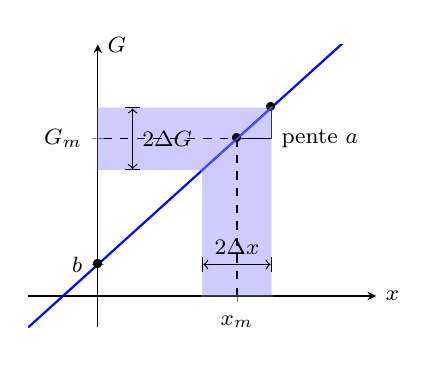
\begin{tikzpicture}
	\begin{axis}[
		width=6cm,
		axis lines=middle,%none,bottom,top
		inner axis line style={=>},
		xlabel={$x$},
		xlabel style={anchor=west},
		ylabel={$G$},
		ylabel style={anchor=west},
		xtick={2},
		xticklabels={$x_\text{m}$},
		x tick label style={below=0.5mm},
		ytick={1,5},
		yticklabels={$b$,$G_\text{m}$},
		xmin=-1,
		xmax=4,
		ymin=-1,
		ymax=8,
		font=\footnotesize,
	]
	\addplot+[thick,mark=none,domain=-1:4,samples=10] {2*x+1};
	\draw[dashed](axis cs:2,0)|-(axis cs:0,5);
	\draw[](axis cs:2,5)node{•}-|(axis cs:2.5,6)node{•}node[midway,right]{pente $a$};	
	\addplot+[thick,mark=none,fill=blue,draw=white,opacity=0.2,domain=1.5:2.5,samples=10]{2*x+1}\closedcycle;
	\draw[fill=blue,opacity=0.2,draw=white](axis cs:0,6)--(axis cs:2.5,6)--(axis cs:1.5,4)--(axis cs:0,4)--cycle;
	\draw[|<->|](axis cs:1.5,1)--(axis cs:2.5,1)node[midway,above]{$2\Delta x$};
	\draw[|<->|](axis cs:0.5,4)--(axis cs:0.5,6)node[midway,right]{$2\Delta G$};
	\draw(axis cs:0,1)node{$\bullet$};
	\end{axis}
\end{tikzpicture}
\caption{Propagation des incertitudes dans le cas d'une relation affine}
\labfig{propagation_affine}
\end{marginfigure}
Dans ce cas, il est facile de voir sur un graphique qu'une incertitude $\Delta x$ produit une incertitude $\Delta G=|a|\Delta x$ de sorte que le calcul donne 
% --- equation --- (fold)
\begin{equation}
\fcolorbox{filet}{fond}{\hspace{0.5em}
\(\displaystyle 
G=G_m\pm\Delta G
\quad\text{avec}\quad
\left\{\begin{array}{rcl}
G_m	&=&ax_\text{m}+b\\
\Delta G&=&|a|\Delta x	
\end{array}\right.
\)\hspace{0.5em}}
\hspace{0.5em}\heartsuit
\label{eq:propagation_erreur_lineaire}
\end{equation}
%--- equation --- (end)

\exercice{L'indice de réfraction de l'air à \(20^\circ \mathrm{C}\) varie avec la pression selon la loi de Gladstone : \(n=1+kP\) avec \(k=(27\pm 1)\cdot 10^{-5}\,\mathrm{bar^{-1}}\) et où \(P\) est exprimé en bar. 
Que vaut l'indice de l'air à \(20^\circ \mathrm{C}\) et à la pression \(P=2\,\mathrm{bar}\) ?\\[2mm]
\emph{Rép.}~~\(n=1,00054\pm 0,00002\).
}
% Le calcul de $n$  et de son incertitude donne \[n=1+27.10^{-5}\times 2=1,00054 \quad\text{et}\quad \Delta n=P\Delta k=2.10^{-5}\] On écrira donc \[n=1,00054\pm0,00002\]


%(end)
\subsection{Cas d'une loi puissance}%(fold)
Supposons maintenant que la grandeur $G$ dépend d'une variable $x$ \emph{via} une loi de puissance :
\[
	G=G_0\,x^n
\]
et cherchons à estimer l'incertitude de $G$ liée à la propagation de l'incertitude de $x$. Pour cela nous allons supposer que les incertitudes sont petites en valeur relative. Cela signifie qu'entre $x$ et $x+\Delta x$, $G$ varie si peu qu'on peut approcher la courbe par un segment de coefficient directeur 
\[
	a=\frac{\mathrm{d}G}{\mathrm{d}x}=n\,G_0\, x^{n-1}
\]
Si l'on applique le résultat du paragraphe précédent, on trouve donc $\Delta G=|a|\,\Delta x=|n\,G_0\,x^{n-1}|\,\Delta x$. En divisant par $G_\text{m}$ on trouve la règle simple suivante.
% --- equation --- (fold)
\begin{equation}
\fcolorbox{filet}{fond}{\hspace{0.5em}
\(\displaystyle 
\left|\frac{\Delta G}{G_\text{m}}\right|=\left|n\frac{\Delta x}{x}\right|
\)\hspace{0.5em}}
\hspace{0.5em}\heartsuit
\end{equation}
%--- equation --- (end)
Dans le cas d'une loi de puissance, l'incertitude relative est multipliée par la puissance.
\begin{kaoexample}[frametitle=Exemple: volume d'une bille]
On cherche à déterminer le volume d'une bille d'acier de rayon $r=(2,778\pm 0,005)\;\mathrm{mm}$. Sachant que le volume d'une sphère s'écrit $V=4/3\pi\,r^3$ on trouve 
\[
	V_\text{m}=89,80\;\mathrm{mm^3}
	\quad\text{et}\quad
	\frac{\Delta V}{V}=3\frac{\Delta r}{r}=0,54\%\quad\Longrightarrow\quad\Delta V=0,5\;\mathrm{mm^3}
\]
On écrira donc $V=(89,8\pm0,5)\;\mathrm{mm^3}$.
\end{kaoexample} 
%(end)
\subsection{Méthode générale}%(fold)
\textbf{\(G\) ne dépend que d'une variable} -- En physique, il arrive souvent que le calcul d'une grandeur $G$ implique plusieurs variables. Cependant, il également assez courant qu'une des variables soit moins précise que les autres de sorte que l'on peut considérer les autres variables comme des paramètres constants. On peut alors considérer que 
\[
G=f(x)	\quad\text{avec}\quad	x=x_m\pm\Delta x
\]
Dans ce cas, et à condition de $G$ varie peu entre $x_m$ et $x_m \pm\Delta x$, on écrira
% --- equation --- (fold)
\begin{equation}
\fcolorbox{filet}{fond}{\hspace{0.5em}
\(\displaystyle 
G=G_m\pm\Delta G
\quad\text{avec}\quad
\left\{\begin{array}{rcl}
G_m	&=&f(x_m)\\
\Delta G&=&\left|f'(x_m)\right|\Delta x	
\end{array}\right.
\)\hspace{0.5em}}
\hspace{0.5em}\heartsuit
\end{equation}
%--- equation --- (end)
\textbf{$G$ dépend de $n$ variables} -- Considérons maintenant le cas général 
\[
G=f(x_1,x_2,\ldots,x_n)	\quad\text{avec}\quad	x_i=x_{\text{m,}i}\pm \Delta x_i
\]
Si les grandeurs $x_i$ sont indépendantes, on utilise la formule suivante  :
\begin{equation}
\fcolorbox{filet}{fond}{\hspace{0.5em}
\(\displaystyle 
\Delta G=\sqrt{(a_1\Delta x_1)^2 + (a_2\Delta x_2)^2+\ldots+(a_n\Delta x_n)^2}
\quad\text{avec}\quad
a_1=\frac{\partial f}{\partial x_1}\ldots
\)\hspace{0.5em}}
\hspace{0.5em}\heartsuit
\label{eq:}
\end{equation}
\begin{kaoexample}[frametitle=Calcul d'une puissance électrique]
Un dipôle électrique est soumis à la tension $U=(2,6\pm0,3)\;\mathrm{V}$ ce qui produit un courant d'intensité $I=(0,89\pm0,06)\;\mathrm{A}$. Calculons la puissance électrique $P=U.I$ fournie à ce dipôle. 

Tout d'abord, la valeur numérique de la puissance vaut 
\[P_\text{m}=U_\text{m}I_\text{m}=2,6\times0,89=2,314\;\mathrm{W}\]
Ensuite, calculons les dérivées par rapport à $U$ et $I$ :
	\[\dfrac{\partial P}{\partial U}=I
	\quad\text{et}\quad
	\dfrac{\partial P}{\partial I}=U
	\quad\Longrightarrow\quad
	\mathrm{d}P=I\, \mathrm{d}U+U\,\mathrm{d}I
	\]
On en déduit l'incertitude sur le calcul de $G$ :
\[
	\Delta P=\sqrt{(0,89\times 0,3)^2+(2,6\times 0,06)^2}=0,31\;\mathrm{W}
\]
On écrira donc :
\[
	P=2,3\pm0,3\;\mathrm{W}
\]
\end{kaoexample} 
%(end)
\subsection{Cas où les données sont fournies sans incertitude}[Données sans incertitude]%(fold)
Il arrive fréquemment, notamment dans les sujets de concours, que l'on ait à faire un calcul à partir de données dont les incertitudes sont absentes. Dans ce cas c'est le nombre de chiffres significatifs qui indique la précision. On admet alors que le dernier chiffre significatif est connu à \(\pm 0{,}5\). Par exemple, 

	\[v=\SI{55}{km.h^{-1}}\quad\text{signifie}\quad v=\SI{55,0\pm 0,5}{km.h^{-1}}\]

Donc, rigoureusement, pour savoir comment arrondir le résultat d'un calcul il faut faire une estimation de l'incertitude liée au calcul. Cependant, si l'on veut s'épargner ce calcul fastidieux, on peut appliquer la méthode simplifiée suivante.

\begin{kaobox}[frametitle={Règles de calcul}]
\begin{itemize}
	\item Cas d'une somme : c'est la donnée qui présente le moins de décimales qui impose son nombre de décimales au résultat.
	\item Cas d'un produit ou d'un quotient : la donnée qui présente le plus faible nombre de chiffres significatifs impose son nombre de chiffres significatif au résultat.
	\item Cas d'une fonction \(f(x)\) : le résultat est arrondi avec le même nombre de chiffres significatifs que \(x\).
\end{itemize}
\end{kaobox} 

\begin{kaoexample}[frametitle=Exemples]
\begin{itemize}
	\item \(25{,}2\,\mathrm{cm}+8{,}3\,\mathrm{mm}=(25{,}2+0{,}83)\,\mathrm{cm}=26{,}0\,\mathrm{cm}\). Le résultat doit être arrondi au dixième de centimètre. Attention à ne pas oublier d'écrire les grandeurs avec la même unité !
	\item \(\dfrac{0{,}600}{0{,}9+0{,}300}=0{,}50\). En effet, la somme 0,9~+~0,300 vaut 1,2 (arrondi au dixième) et possède deux chiffres significatifs. Le résultat doit présenter deux chiffres significatifs.
	\item \(\dfrac{0{,}300\times 4{,}180\times(15-7{,}0)}{0{,}069}=145,39\ldots\simeq 1.10^3\), car \(15-7{,}0=8\) est arrondi à l'unité près et ne présente donc qu'un seul chiffre significatif.
\end{itemize}
\end{kaoexample} 


%(end)

%(end)
